\documentclass[12pt]{article}
\usepackage[english]{babel}
\usepackage[T1]{fontenc}
\usepackage[utf8]{inputenc}
\usepackage{amssymb}
\usepackage{amsmath}
\usepackage{graphicx}
\usepackage{hyperref}
\newcommand{\pat}{\partial}
\newcommand{\be}{\begin{equation}}
\newcommand{\ee}{\end{equation}}
\newcommand{\bea}{\begin{eqnarray}}
\newcommand{\eea}{\end{eqnarray}}
\newcommand{\abf}{{\bf a}}
\newcommand{\Zcal}{{\cal Z}_{12}}
\newcommand{\zcal}{z_{12}}
\newcommand{\Acal}{{\cal A}}
\newcommand{\Fcal}{{\cal F}}
\newcommand{\Ucal}{{\cal U}}
\newcommand{\Vcal}{{\cal V}}
\newcommand{\Ocal}{{\cal O}}
\newcommand{\Rcal}{{\cal R}}
\newcommand{\Scal}{{\cal S}}
\newcommand{\Lcal}{{\cal L}}
\newcommand{\Hcal}{{\cal H}}
\newcommand{\hsf}{{\sf h}}
\newcommand{\half}{\frac{1}{2}}
\newcommand{\Xbar}{\bar{X}}
\newcommand{\xibar}{\bar{\xi }}
\newcommand{\barh}{\bar{h}}
\newcommand{\Ubar}{\bar{\cal U}}
\newcommand{\Vbar}{\bar{\cal V}}
\newcommand{\Fbar}{\bar{F}}
\newcommand{\zbar}{\bar{z}}
\newcommand{\wbar}{\bar{w}}
\newcommand{\zbarhat}{\hat{\bar{z}}}
\newcommand{\wbarhat}{\hat{\bar{w}}}
\newcommand{\wbartilde}{\tilde{\bar{w}}}
\newcommand{\barone}{\bar{1}}
\newcommand{\bartwo}{\bar{2}}
\newcommand{\nbyn}{N \times N}
\newcommand{\repres}{\leftrightarrow}
\newcommand{\Tr}{{\rm Tr}}
\newcommand{\tr}{{\rm tr}}
\newcommand{\ninfty}{N \rightarrow \infty}
\newcommand{\unitk}{{\bf 1}_k}
\newcommand{\unitm}{{\bf 1}}
\newcommand{\zerom}{{\bf 0}}
\newcommand{\unittwo}{{\bf 1}_2}
\newcommand{\holo}{{\cal U}}
\newcommand{\bra}{\langle}
\newcommand{\ket}{\rangle}
\newcommand{\muhat}{\hat{\mu}}
\newcommand{\nuhat}{\hat{\nu}}
\newcommand{\rhat}{\hat{r}}
\newcommand{\phat}{\hat{\phi}}
\newcommand{\that}{\hat{t}}
\newcommand{\shat}{\hat{s}}
\newcommand{\zhat}{\hat{z}}
\newcommand{\what}{\hat{w}}
\newcommand{\sgamma}{\sqrt{\gamma}}
\newcommand{\bfE}{{\bf E}}
\newcommand{\bfB}{{\bf B}}
\newcommand{\bfM}{{\bf M}}
\newcommand{\cl} {\cal l}
\newcommand{\ctilde}{\tilde{\chi}}
\newcommand{\ttilde}{\tilde{t}}
\newcommand{\ptilde}{\tilde{\phi}}
\newcommand{\utilde}{\tilde{u}}
\newcommand{\vtilde}{\tilde{v}}
\newcommand{\wtilde}{\tilde{w}}
\newcommand{\ztilde}{\tilde{z}}


\hoffset 0.5cm
\voffset -0.4cm
\evensidemargin -0.2in
\oddsidemargin -0.2in
\topmargin -0.2in
\textwidth 6.3in
\textheight 8.4in

\begin{document}

\normalsize

\baselineskip 14pt

\begin{center}
{\Large {\bf FYMM/MMP IIIb 2020 \ \ \  Solutions to Problem Set 3}}
Jake Muff
\end{center}



\begin{enumerate}
    \item Question 1. We have 
    $$ f: S^1 \rightarrow S^2 $$ 
    \begin{enumerate}
        \item From page 45 of the lecture notes we have 
        $$ X = X^{\mu} \frac{\partial}{\partial x^{\mu}} $$
        And from page 51 of the elcture notes we have 
        $$ f_* X = X^{\mu} \frac{\partial y^{\alpha}}{\partial x^{\mu}} \frac{\partial}{\partial y^{\alpha}} $$
        Following the example of page 51 we have 
        $$ x^1 = \phi; y^1 = \theta, y^2 = \varphi $$ 
        $$ V = \dot{\phi}(t) \frac{\partial}{\partial \phi} $$ 
        $$ X = V, X^{\mu} = \dot{\phi}(t), \frac{\partial y^{\alpha}}{\partial x^{\mu}} = \frac{\partial \theta}{\partial \phi} = \frac{1}{2} $$
        $$ \frac{\partial}{\partial y^{\alpha}} = \frac{\partial \varphi}{\partial \phi} = 1 $$
        So 
        $$ f_* V = \dot{\phi} ( \frac{1}{2} \frac{\partial}{\partial \theta} + \frac{\partial}{\partial \varphi} ) $$
        Overall, for $c(t) = \phi (t) = at$ 
        $$ \dot{\phi} = a $$
        $$ V = a \frac{\partial}{\partial \phi} $$
        So 
        $$ f_* V = a( \frac{1}{2} \frac{\partial}{\partial \theta} + \frac{\partial}{\partial \varphi} ) $$

        \item $c(t) = \phi (t) = 2 \pi \sin (t) $ we have 
        $$ \dot{\phi} = 2 \pi \cos(t)  $$
        $$ V = 2 \pi \cos (t) \frac{\partial}{\partial \phi} $$
        $$ f_* V = 2 \pi \cos (t) ( \frac{1}{2} \frac{\partial}{\partial \theta} + \frac{\partial}{\partial \varphi}) $$

    \end{enumerate}

    \item Following pg 53, Proving that $XY$ is not a vector field. If we have two smooth vector fields $X$ and $Y$ and we apply $XY$ to the smooth function $f$ acting on $M$ we would have 
    $$ XYf = ( X^{\mu} \partial_{\mu} Y^{\mu} \partial_{\mu} ) f= X^{\mu} \partial_{\mu} \Big[ Y^{\nu} \partial_{\nu} f \Big] $$
    $$ = X^{\mu} \partial_{\mu}  Y^{\mu} \partial_{\mu} f + X^{\mu} Y^{\mu} ( \partial_{\mu} \partial_{\mu} f) $$
    $$ = X^{\mu} ( \partial_{\mu} Y^{nu} ) \partial_{\nu} f + X^{\mu} Y^{\nu} \partial_{\mu} \partial_{\nu} f $$
    The first term is a vector field but the second is not as we cannot write $XY$ as a function of $Z$ i.e $XYf = Z^{\mu} \partial_{\mu} f $.
    \\
    Showing that $[X,Y]$ is a smooth vector field, we apply the same method as before 
    $$ [X,Y]f = XYf - YXf $$
    $$ = X^{\mu} (\partial_{\mu} Y^{\nu} ) \partial_{\nu} f + X^{\mu} Y^{\nu} ( \partial_{\mu} \partial_{\nu} f) -  (Y^{\mu} ( \partial_{\mu} X^{\nu} ) \partial_{\nu} f + Y^{\mu} X^{\nu} ( \partial_{\mu} \partial_{\nu} f)) $$
    $$ = X^{\mu} ( \partial_{\mu} Y^{\nu} ) \partial_{\nu} f - Y^{\mu} ( \partial_{\mu} X^{\nu} ) \partial_{nu} f $$
    Both terms are vector fields and satisfy 
    $$ [X,Y]f = Z^{\mu} \partial_{\mu} f $$
    So $[X,Y]$ is a smooth vector field. 
    \\
    To prove the first identity we have 
    $$ [X,fY] = X(fY) - (fY)X $$
    $$ = XfY + fXY - fYX $$
    $$ = (Xf)Y + f[X,Y] $$
    To prove the second identity:
    $$ [X,[Y,Z]] + [Z,[X,Y]] + [Y, [Z,X]] = $$
    $$ = XYZ - XZY - YZX + ZYX + YZX - YXZ - ZXY+ XZY + ZXY - ZYX - XYZ + YXZ $$
    $$ = 0 $$
    
    \item Hamilton's equations as an example of a flow generated by a vector field. 
    $$ H: M \rightarrow \mathbb{R} $$
    \begin{enumerate}
        \item Vector field $X_H$ gives integral curves 
        $$ x_H (t) = \textrm{ the basis}\ \mu \rightleftarrows i $$
        $$ \dot{x}_H^{\mu} = X^{\mu}_H$$
        For $\mu = 1 \ldots N$. So we have 
        $$ \frac{\partial q_i}{\partial t} = -\frac{\partial H}{\partial p_i} $$
        Holds for $\mu = N+1 \ldots 2N$. Thus the integral curves for $x_H (t) $ are equivalent to the Hamiltonian equations of motion. 

        \item We have $M = \mathbb{R}^2 \rightarrow N=1, H= \frac{1}{2} ( p^2 + q^2) $. This means that 
        $$ X_H = \frac{\partial H}{\partial p} \frac{\partial}{\partial q} - \frac{\partial H}{\partial q} \frac{\partial}{\partial p} $$
        $$ = \frac{\partial}{\partial p} ( \frac{1}{2} ( p^2 + q^2)) \frac{\partial}{\partial q} - \frac{\partial}{\partial q} (\frac{1}{2} (p^2 + q^2 )) \frac{\partial}{\partial p} $$
        $$ = p \frac{\partial}{\partial q} - q \frac{\partial}{\partial p} $$
        So we need to solve 
        $$ \dot{q} = p, \dot{p} = - q $$
        With $q(0) =1, p(0) =0$. Using wolffram alpha we get 
        $$ p(t) = - \sin (t) $$
        $$ q (t) = \cos (t) $$
        \begin{figure}[h]
            
            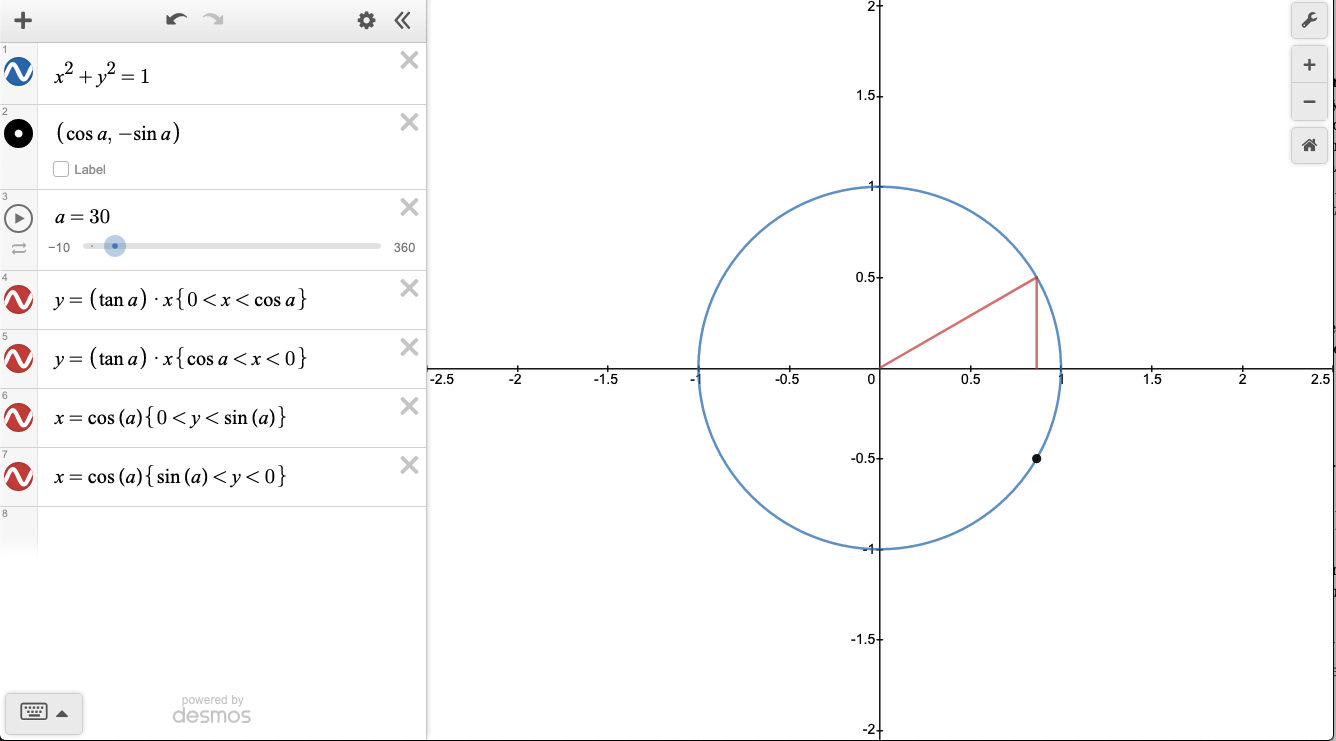
\includegraphics[width=15cm]{desmos1.png}
            \centering
            \caption{The differential equations describe a unit circle but with clockwise rotation. This figure shows the desmos representation of this. }
        \end{figure}

        \item Now with $H = \frac{1}{2} (p^2 - q^2)$ and $x_0 = (1,1)$ So we have 
        $$ X_H = p \frac{\partial}{\partial q} + q \frac{\partial}{\partial p} $$
        The differential equations are then 
        $$ \dot{q} = p, \dot{p} = q $$
        With 
        $$ q(0) =1, p(0) =1 $$
        Solved using wolffram alpha
        $$ p(t) = e^t $$
        $$ q(t) = e^t $$ 
        Which is a straight line. 

        \item $M = T^2$, $T^2$ is the 2-torus. $H = \cos (p)$. 
        $$ X_H = \frac{\partial}{\partial p} ( \cos (p) ) \frac{\partial}{\partial q} - \frac{\partial}{\partial q} ( \cos (p)) \frac{\partial}{\partial p} $$
        $$ = - \sin (p) \frac{\partial}{\partial q} - 0 $$
        Solved using wolffram alhpa gives 
        $$ \dot{q} = - \sin (p), \dot{p} = 0 $$
        $$ p(t) = c_1 $$
        Where $c_1$ is a constnat or would equal the initial conditions. 
        $$ q(t) = c_2 - t \sin (c_2) $$
        I don't know how this would look exactly but $q(t)$ is a striahgt line around $q$ which is the case of a 2-torus, $q$ would be the angle and $q(t)$ would be a straight line on $T^2$. 


    \end{enumerate}

    \item The vector field 
    $$ X = X^{\mu} (x) \frac{\partial}{\partial x^{\mu}} $$
    $$ g = g_{\mu \nu} (x) d x^{\mu} \otimes dx^{\nu} $$
    The lie derivative $L_X g$ would therefore be (following Lecture notes) 
    $$ L_X g = (L_x g_{\mu \nu} ) dx^{\mu} \otimes dx^{\nu} + g_{\mu \nu} ( L_X dx^{\mu} ) \otimes dx^{\nu} + g_{\mu \nu} dx^{\mu} \otimes (L_X dx^{\nu} ) $$
    $$ = ( X^{\alpha} \partial_{\alpha} g_{\mu \nu} ) dx^{\mu} \otimes dx^{\nu} + g_{\mu \nu} ( \partial_{\alpha} X^{\mu} ) dx^{\alpha} \otimes dx^{\nu} + g_{\mu \nu} dx^{\mu} \otimes \partial_{\alpha} X^{\alpha} dx^{\alpha} $$
    

\end{enumerate}



\end{document}
